\documentclass{standalone}
\usepackage{tikz}
\usepackage{ctex,siunitx}
\usepackage{tkz-euclide}
\usepackage{amsmath}
\usetikzlibrary{patterns, calc}
\usetikzlibrary {decorations.pathmorphing, decorations.pathreplacing, decorations.shapes,}
\begin{document}
\small
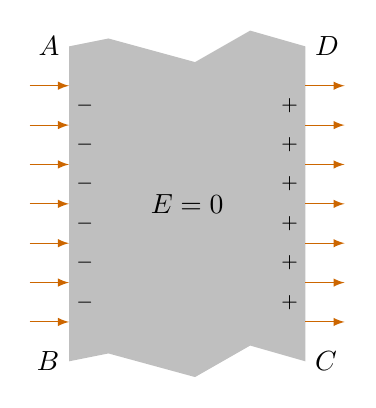
\begin{tikzpicture}[>=latex,scale=1.0]
  % \useasboundingbox(-1,-2)rectangle(8,6);
  \fill[lightgray](-1.5,-2)--(-1.0,-1.9)--(0.1,-2.2)--(0.8,-1.8)--(1.5,-2)--(1.5,2)--(0.8,2.2)--(0.1,1.8)--(-1.0,2.1)--(-1.5,2)--cycle;
  \foreach \x in {-1.5,-1.0,...,1.5}
  {
    \draw[orange!80!black,->](-2,\x)--(-1.5,\x);
    \draw[orange!80!black,->](1.5,\x)--(2,\x);
  }
  \node at (-1.5,2) [left]{$A$};
  \node at (-1.5,-2)[left]{$B$};
  \node at (1.5,-2)[right]{$C$};
  \node at (1.5,2)[right]{$D$};
  \foreach \x in {-1.25,-0.75,...,1.25}
  {
    \node at (1.3,\x) {\scriptsize $+$};
    \node at (-1.3,\x) {\scriptsize $-$};
  }
  \node at (0,0){$E=0$};
\end{tikzpicture}
\end{document}